\documentclass{report}

\usepackage[a4paper, total={6in, 8in}, margin=1in,footskip=0.25in]{geometry}
\usepackage{amsmath, amsthm, amssymb, booktabs, chemfig, graphicx, float, pgfplots, setspace, siunitx, tabularray}
\usepackage{tabularray}
\usepackage[hidelinks]{hyperref}

\setlength{\parindent}{0pt}
\setlength{\parskip}{0.8em}

\pgfplotsset{compat=1.18}

\graphicspath{ {.././Images/} }

\title{\Huge Year 12 Physics}
\author{L. Cheung}

\tolerance=1
\emergencystretch=\maxdimen
\hyphenpenalty=10000
\hbadness=10000

\begin{document}
	\maketitle
	\tableofcontents
\newpage

\chapter{Investigations}

	\section{Investigation 1: Speed of Light Investigations}
	
		\textbf{Summarise the historical and contemporary methods used to determine the speed of light and explain its current relationship to the measurement of time and distance.}
		
		

\newpage

	\section{Investigation 2: Spectral Analysis}
	
		\textbf{Aim}: To determine the emission spectra of various elements

		\subsubsection{Materials}
		
			\begin{itemize}
				\item Spectroscope
				\item Spectral lamps with:
					\begin{itemize}
						\item Hydrogen
						\item Helium
						\item Neon
						\item Oxygen
						\item Mercury
					\end{itemize}
				\item Spectral lamp support
				\item Spectral lamp power supply
			\end{itemize}

		\subsubsection{Risk Assessment}

			\begin{table}[H]
				\setstretch{1.25}
				\centering
				\begin{tabular}{p{7cm}|p{7cm}}
					\textbf{Hazard} & \textbf{Precaution} \\ \hline
					High voltage power pack & Turn off when not in use, do not touch contact points \\
					Cuts from glass & Check spectral lamp before use, keep away from edge of table to prevent dropping \\
					Burns from UV light & Don't observe directly, only view via spectrometer
					
				\end{tabular}
			\end{table}

		\subsubsection{Method}
			\begin{enumerate}
				\item Prepare spectral support and power supply at 400V
				\item Insert hydrogen spectral
				\item Use spectrometer to observe emission spectrum and record wavelengths using chart on spectrometer
				\item Repeat steps 2-3 with helium, neon, sulfur, and mercury
				\item Record results
			\end{enumerate}

		\subsubsection{Results}
			\begin{table}[H]
				\centering
				\setstretch{1.25}
				\begin{tabular}{p{3cm}|p{10cm}}
					\textbf{Element}	& \textbf{Result}			\\ \hline
					Hydrogen		& Bright pink				\\
					Helium			& Red, orange, yellow			\\
					Neon			& Red, orange				\\
					Oxygen			& Pale blue white			\\
					Mercury			& Blue-green				\\
				\end{tabular}
			\end{table}

\newpage

	\section{Investigation 3: Diffraction of Light}
	
		\textbf{Summarise your qualitative analysis of light diffraction, including the experimental setup, observations, and what these phenomena demonstrate about the wave properties of light.}

\newpage

	\section{Investigation 4: Interference and Diffraction}

		\textbf{Aim}: To observe the diffraction and interference of light using diffraction gratings
		\subsubsection{Materials}

			\begin{itemize}
				\item Laser pointer
				\item A diffraction grating set
				\item Meter ruler or tape measure
			\end{itemize}

		\subsubsection{Risk Assessment}
		
			\begin{table}[H]
				\setstretch{1.25}
				\centering
				\begin{tabular}{p{7cm}|p{7cm}}
					\textbf{Hazard} & \textbf{Precaution} \\ \hline
					Retina burns & Do not directly look at laser light \\
					Dropping equipment & Handle with caution, keep secure on table

				\end{tabular}
			\end{table}
		
		\subsubsection{Method}

			\begin{enumerate}
				\item Use supports such as retort stands to set up the laser pointer so that it shines perpendicularly onto a screen, wall, or board at least one meter away.
				\item Mount the diffraction grating directly in front of the laser pointer so that a regular row of dots appears on the screen.
				\item Measure the values of $x$ and $L$, and record these in your results table, along with the $N$ value for your grating.
				\item Repeat this procedure for each grating of different $N$ value.
				\item Analyse the data to determine the wavelength of the laser pointer.
			\end{enumerate}

		\subsubsection{Results}

			\begin{figure}[H]
				\centering
				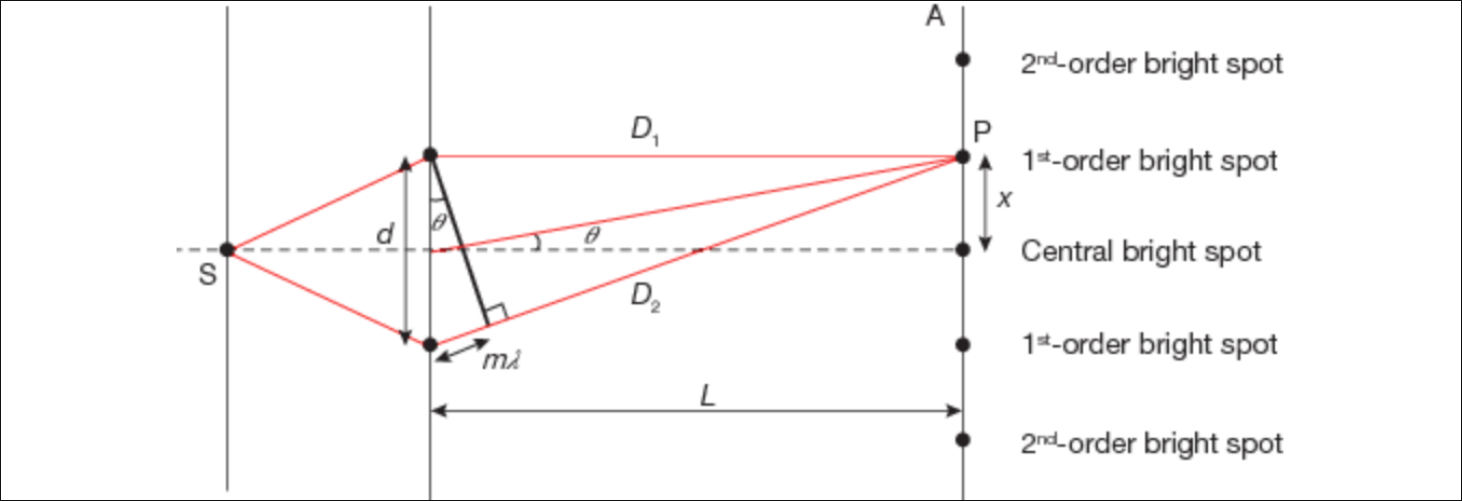
\includegraphics[width=15cm]{young_double_slit.png}
			\end{figure}

			\begin{table}[H]
				\centering
				\setstretch{1.25}
				\begin{tabular}{p{4cm}|p{2cm}|p{2cm}|p{2cm}|p{2cm}}
					Slit separation $d$ (m)		& $x$ (m)	& L (m)		& $\lambda$ (m) 		& $\lambda$ (nm)	\\ \hline
					$100 \times 10^{-6}$		& 0.034		& 5.44		& $6.25 \times 10^{-7}$		& 625			\\
					$200 \times 10^{-6}$		& 0.016		& 5.44		& $5.88 \times 10^{-7}$		& 588			\\
					$300 \times 10^{-6}$		& 0.011		& 5.44		& $6.07 \times 10^{-7}$		& 607			\\
				\end{tabular}
			\end{table}
			
			Slit separation 1
			\begin{align*}
				\text{At very small angles, } \sin{\theta} = \tan{\theta} \\
				d \sin{\theta} &= m \lambda \\
				\sin{\theta} = \frac{m \lambda}{d} &= \frac{x}{L} \\
				\lambda &= \frac{dx}{L} \\
					&= \frac{100 \times 10^{-6} \times 0.034}{5.44} \\
					&= 6.25 \times 10^{-7} \\
			\text{Actual $\lambda$ of Ne-He laser} &= 6.328 \times 10^{-7}
			\end{align*}

			Slit separation 2
			\begin{align*}
				d \sin{\theta} &= m \lambda \\
				\sin{\theta} = \frac{m \lambda}{d} &= \frac{x}{L} \\
				\lambda &= \frac{dx}{L} \\
					&= \frac{200 \times 10^{-6} \times 0.016}{5.44} \\
					&= 5.88 \times 10^{-7} \\
			\text{Actual $\lambda$ of Ne-He laser} &= 6.328 \times 10^{-7}
			\end{align*}

			Slit separation 3
			\begin{align*}
				d \sin{\theta} &= m \lambda \\
				\sin{\theta} = \frac{m \lambda}{d} &= \frac{x}{L} \\
				\lambda &= \frac{dx}{L} \\
					&= \frac{300 \times 10^{-6} \times 0.011}{5.44} \\
					&= 6.07 \times 10^{-7} \\
			\text{Actual $\lambda$ of Ne-He laser} &= 6.328 \times 10^{-7}
			\end{align*}
\newpage

\chapter{Review Questions}

	\section{Electromagnetic Spectrum}

		\begin{enumerate}
			\item B
			\item D
			\item B
			\item C
			\item A
			\item \textbf{Figure 8.11 shows the emission spectrum of sodium}
				\begin{enumerate}
					\item \textbf{Describe an experiment that could be used to examine the emission spectrum of an element.}
						\subitem The spectral lamp experiment can be used to observe the emission spectrum of an element. Running high voltage current through a spectral lamp containing a specific element will emit a bright spectrum that can be split into wavelengths by a prism or a spectrocope.

					\item \textbf{Explain how emission spectra can be used to identify the elements in a sample?}
						\subitem A complete emission spectra can be analysed to find the lines in the black body spectrum and comparing that with the spectra of known elements.

					\item \textbf{If sodium was present in the atmosphere of the Sun, how would it affect the emission spectra of the Sun?}
						\subitem If sodium is present, the Sun's emission spectrum will have lines at 589 nm to 590 nm.
				\end{enumerate}

			\item \textbf{Outline one method that has been used to measure the speed of light}
				\subitem Leon Foucault measured the speed of light using a light
		\end{enumerate}

\end{document}

